\documentclass[a4paper,11pt]{article}
\usepackage[left=2cm,text={17cm, 24cm},top=3cm]{geometry}
\usepackage[utf8]{inputenc}
\usepackage[czech]{babel}
\usepackage{times}
\usepackage[hidelinks]{hyperref}
\usepackage{graphicx}
\usepackage{booktabs}
\usepackage{epstopdf}
\usepackage{fancyvrb}
\usepackage{amsmath}
\usepackage{float}
\fvset{frame=single,framesep=1mm,fontfamily=courier,fontsize=\scriptsize,numbers=left,framerule=.3mm,numbersep=1mm,commandchars=\\\{\}}
\usepackage[usenames,dvipsnames]{xcolor}
\graphicspath{{./images/}}
\usepackage{listings}
\lstdefinestyle{customc}{
	abovecaptionskip=0\baselineskip,
	breaklines=true,
	frame=L,
	xleftmargin=\parindent,
	language=C,
	showstringspaces=false,
	basicstyle=\footnotesize\ttfamily,
	keywordstyle=\bfseries\color{green!40!black},
	commentstyle=\itshape\color{purple!40!black},
	identifierstyle=\color{blue},
	stringstyle=\color{orange},
	captionpos=b
}
\renewcommand{\lstlistingname}{Kód}
\lstset{escapechar=@,style=customc}

\begin{document}
\begin{center}
\Huge
\textsc{Vysoké učení technické v~Brně\\
}Fakulta informačních technologií\\
\vspace{\stretch{0.382}}
\LARGE Implementace interpretu imperativního jazyka IFJ16 \\
\Huge Tým 021, varianta a/3/I\\
\vspace{\stretch{0.309}}

\Large Vedoucí:	Kyzlink Jiří 	(xkyzli02)\\
				Kubiš Juraj		(xkubis15)\\
				Korček Juraj	(xkorce01)\\
				Kubica Jan		(xkubic39)\\
				Kovařík Viktor	(xkovar77)\\

\vspace{\stretch{0.309}}

\end{center}
{\Large \today \hfill
Brno}
\thispagestyle{empty}

\newpage

\tableofcontents

\newpage
\section{Úvod}
V této dokumentaci naleznete popis návrhu a implementace interpretu jazyka IFJ16, který je velmi zjednodušenou podmnožinou jazyka Java SE 8, což je staticky typovaný objektově orientovaný jazyk. Vybrali jsme si variantu  a/3/I, což znamená, že funkce find využívá Knuth-Morris-Prattův algoritmus, ve funkci sort je použit řadící algoritmus \texttt{shell sort} a tabulka symbolů je implementovaná binárním vyhledávacím stromem.

--bude ještě doplněno-

\section{Lexikální analyzátor}
Lexikální analýza je založena na deterministickém konečném automatu (dále jen \textit{KA}), jehož vstupem je zdrojový kód programu. Lexikální analyzátor na základě předem definovaných pravidel rozdělí jednotlivé posloupnosti znaků na lexémy, které jsou vráceny syntaktickému analyzátoru ve formě tokenů. Token obsahuje informace o typu rozpoznaného lexému, jeho délce, pozici ve zdrojovém kódu a odpovídající řetězec ze zdrojového kódu. Vedlejším úkolem lexikální analýzy je odstraňování bílých znaků, řádkových i blokových komentářů. Lexikální analýza je řízena syntaktickou analýzou, která postupně žádá o tokeny. Naše implementace obsahuje funkci \texttt{peek\_token}, která umožňuje syntaktické analýze podívat se na další tokeny, bez jejich konzumace. Jména identifikátorů jsou porovnána s prvky v poli řetězců, které obsahuje klíčová slova.

Pokud lexikální analýza narazí na nerozpoznatelný lexém, vypíše na chybový výstup hlášení o chybě, které obsahuje mimo jiné i řádek ve zdrojovém souboru na kterém se vyskytla.

Diagramy konečného automatu lexikálního analyzátoru jsou v \hyperref[diag:LA-FSM]{příloze}.


\section{Syntaktický analyzátor}
Syntaktický analyzátor (dále jen \textit{SA}) slouží k vyhodnocování správnosti syntaxe a v našem případě i ke generování abstraktního syntaktického stromu (dále jen \textit{AST}). Vstupen SA je proud tokenů z LA, výstupem je \hyperref[lst:saOut]{struktura} na listingu níže. Struktura obsahuje tybulku globálních symbolů, pro případ kontroly typů, seznam definovaných funkcí, kde každá obsahuje vlastní AST a v posledním prvku je uložen počet globální proměnných pro potřeby alokace paměti.

\begin{lstlisting}[caption={Výstupní struktura SA}, label={lst:saOut}]
typedef struct {
	Symbo_tree global_symbols;
	Function_list functions;
	int globals;
} Syntax_context;
\end{lstlisting}

\subsection{Syntaktická analýza kódu}
Syntaktická analýza kódu je implementovaná pomocí rekurzivního sestupu

\subsection{Syntaktická analýza výrazů}
Úkolem syntaktickýho analyzátoru výrazů je správně trasformovat výraz na vstupe z formy sledu tokenů do formy AST. Při této trasformaci se musí řídit prioritou a asociatovitou jednotlivých operátorů.

Celej analyzátor se dá rozdělit na tři základní časti: zásobník, množina pravidel a přecedenční tabulka operátorů (dále jen \textit{tabulka}). Analýza probíha způsobem, že jsou všechny vstupní tokeny postupne vkládány na zásobník a redukovány na neterminály na základe pravidel. Kdy a jaká akce se vykoná, se rozhoduje na základe tabulky, ve které se vyhladá relace medzi vstupním tokenem a tokenem (neterminálem), který leží na zásobníku nejblíže vrcholu. Analýza končí, pokud na vstupu prečteme token značíci konec výrazu a na zásobníku se nenachází žádnej neterminál a pouze jeden terminál.

\subsubsection{Precedenční tabulka operátorů}
Tahle tabulka vyjadruje vztah (relaci) medzi každou dvojicí operátorů. Tyhle relace zohladňují vzájemnou prioritu i asociativitu operátorů a určují akci, která se na zásobníku vykoná. Tahle akce může být: 
\begin{itemize}
   \item Vložení vstupního tokenu na zásobník a načtení dalšího tokenu \textit{(v tabulce symbol =)}
   \item Vložení zarážky na vrchol zásobníku, následné vložení vstupního tokenu na zásobník a načtení dalšího tokenu \textit{(v tabulce symbol \textless)}
   \item Záměna tokenů (neterminálů) od zarážky po vrchol zásobníku za jeden terminál \textit{(v tabulce symbol \textgreater)}
   \item Spracování volání funkce (obnáší přečtení dalších tokenů na vstupu) a nahrazení tokenů od zarážky výše za odpovídajíci terminál \textit{(v tabulce symbol F)}
\end{itemize}

Pokud má relace dvou operátorů v tabulce označení \textit{E}, znamená to, že takové vzájemné postavení tychto operátorů netvoří validní výraz a tudiž se jendá o chybu.

\subsubsection{Pravidla}
Jedna z akcí provádených na zásobníku je redukce jedného či více tokenů (neterminálů) na jeden terminál. Pokud je pro tuto redukci zavedené pravidlo, je na jeho základu vykonána, pokud ne, jedná se opět o chybu. V našem projektu jsou použita nasledujíci pravidla:

\begin{align*}
E &\rightarrow E + E  &   E &\rightarrow E < E\\
E &\rightarrow E - E  &   E &\rightarrow E > E\\
E &\rightarrow E * E  &   E &\rightarrow E <= E\\
E &\rightarrow E / E  &   E &\rightarrow E >= E\\
E &\rightarrow ( E )  &   E &\rightarrow E == E\\
E &\rightarrow i      &   E &\rightarrow E != E\\
\end{align*}

\subsubsection{Zásobník}
Je to pracovní entita, ve které je uchovávan rozpracovaný výraz a všechny ostatní informace potrebné pro analýzu. Pro naše účely jsme navrhli zásobník, který má následovní struktúru:

\begin{lstlisting}[caption={Výstupní struktura SA}, label={lst:saOut}]
typedef enum {
    EOS,
    TOKEN,
    EXPRESSION
} t_Element_Type;

typedef struct {
    t_Element_Type type;
    void* address;
    int stop_bit;
} t_Element;

typedef struct {
    t_Element* arr;
    int stack_size;
    int top_element;
    int top_token;
} t_Stack;

\end{lstlisting}


\section{Sémantický analyzátor}


\section{Interpret}

\section{Vestavěné funkce}
Vestavěné funkce jsou pro přehlednost rozděleny na dvě části, neboť podle zadání musí být funkce \texttt{find} a \texttt{sort} uloženy právě v souboru \texttt{ial.c}. Ostatní funkce jsou k nalezení v souboru \texttt{build\_in.c}.

\subsection {vestavěné funkce v IAL.c}
--nevím jestli rozdělovat na podsekce ještě měnší nebo ne--

\subsubsection {\texttt{int find(String s, String search)}}
Funkce \texttt{int find(String s, String search)} hledá první výskyt zadaného podřetězce (v parametru \texttt{search}) a vrátí jeho pozici (počítanou od nuly). V naší variantě a/3/I jsme měli za úkol implementovat tuto funkci pomocí \texttt{Knuth-Morris-Prattova algorytmu}. Tato implementace spočívala v ... doplním.

\subsubsection {\texttt{String sort(String s)}}
Funkce \texttt{String sort(String s)} řadí parametrem daný řetězec \texttt{s} podle ordinální hodnoty obsažených znaků, který pak odevzdává návratovou hodnotou. Daný výpočet je dle zadání a/3/I zpracován pomocí řadícího algoritmu \texttt{Shell sort}, nebo též řazení se snižujícím se přírůstkem s asymptotickou složitostí $O(n^{2})$. Styl implementace vychází ze vzorového příkladu přednášek předmětu IAL, kdy při prvním průchodu je brán krok jakožto polovina počtu prvků z celkové délky řetězce.

\subsection {vestavěné funkce v souboru build{\_}in.c}
Pro usnadnění práce při interpretaci jsou zde u funkcí návratové typy zjednodušeny na datový typ \texttt{Value} a parametry funkcí jsou předávány pomocí datového typu \texttt{Value\_list}.

\begin{itemize}
\item {\texttt{int readInt ()}} - funkce zpracovává čtený řetězec ze standardního vstupu po znacích a je zde tak zřejmá podobnost s konečnými automaty. Při nepovoleném znaku pro datový typ \texttt{int} volá funkce ke konci chybové hlášení, jinak je připuštěno k převodu řetězce na celé číslo.
\item {\texttt{double readDouble ()}} - funkce je charakterem obdobná s funkci \texttt{readInt} a výsledná kontrola na desetinné číslo je ošetřena pomocí céčkové funkce \texttt{strtod()}.
\item {\texttt{String readString ()}} - funkce na podobném přístupu jako \texttt{readInt} s rozšířenou množinou povolených znaků.
\item {\texttt{void print ( \emph{term\_nebo\_konkatenace} )}} - funkce tisknoucí svůj vstup na standartní výstup. Zde je ošetřena možnost proměnného počtu parametrů pomocí datového typu \texttt{Value\_list}. 
\item {\texttt{int length(String s)}} - funkce pro zjištění délky daného řetězce, která sama vychází z céčkové funkce \texttt{strlen()}.
\item {\texttt{String substr(String s, int i, int n)}} - funkce tiskne podřetězec daného řetězce \texttt{s} s ošetřením na přesah paměti pomocí céčkové funkce \texttt{strncat()}.
\item {\texttt{int compare(String s1, String s2)}} - funkce porovnává dva dané řetězce na základě céčkové funkce \texttt{strcmp()}.
\end{itemize}

\section{Testy}
Testovali jsme buď součásti - \textit{unit testy}, kde jsme zkoušeli, zda daná funkce správně reaguje na vstupy. Unit testy si dělal každý sám a podle potřeby. Bylo zvykem v Makefile pro unit test udělat zvláštní target, kde se kromě samotné kompilace ještě prováděl \textit{valgrind} test pro ověření možných \textit{memory leaků}. 

Dále jsme dělali ještě systémové testy. To byly vlastně testy samotného interpretu a porovnávání jeho výstupu s výstupem Javy SE 8 s přidanou kompatibilitou s jazykem IFJ16. Test byl vytvořen jako samostatný bash script, který se volal z Makefile. Ve složce test/input/ byly různé programy v jazyce IFJ16 ve formátu \textit{návratovýKód\_názevProgramu.ifj16} s možností přidání ještě souboru se stejným formátem, ale koncovkou .in, kde byla možnost dát vstup na \textit{stdin}. Daný skript pak prošel složku, zjistil, zda jsou v ní obsaženy i soubory typu .in pro právě interpretovaný kód. Pokud byla předpokládaná návratová hodnota 0 (chyby IFJ16 interpretu nemělo smysl překládat v Javě a porovnávat), došlo k interpretaci kódu v Javě i ifj16 interpretu s následným porovnání návratových kódů a výstupů. Vše se zapisovalo do logu, který se nacházel ve stejné složce \textit{input} jako interpretovaný kód. Obrázek níže zobrazuje výsledky testování v průběhu raných fází interpretu.\\


%\begin{figure}
%	\centering
%	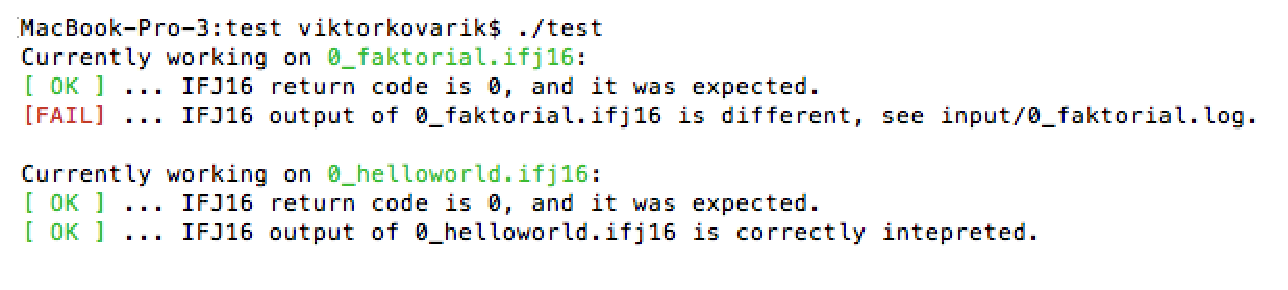
\includegraphics[width=0.7\linewidth]{testy-interpretu.eps}
%	\caption{}
%	\label{fig:testy-interpretu}
%\end{figure}

\begin{Verbatim}
ciUser@travis: ./test
Currently working on 0_ahojsvete.ifj16:
\textbf{\color{green}[ OK ]} ... IFJ16 return code is 0, and it was expected.
\textbf{\color{green}[ OK ]} ... IFJ16 output of 0_ahojsvete.ifj16 is correctly intepreted.

Currently working on 0_arithmetic_test_9_UNARY.ifj16:
\textbf{\color{red}[FAIL]} ... IFJ16 return code is 2, but 0 was expected, see logs/0_fooTest.log.
\textbf{\color{red}[FAIL]} ... IFJ16 output of 0_fooTest.ifj16 is different, see logs/0_fooTest.log.
\end{Verbatim}


\section{Přílohy}
\subsection{Diagramy konečného automatu lexikální analýzy}
\label{diag:LA-FSM}
\begin{figure}[H]
	\centering
	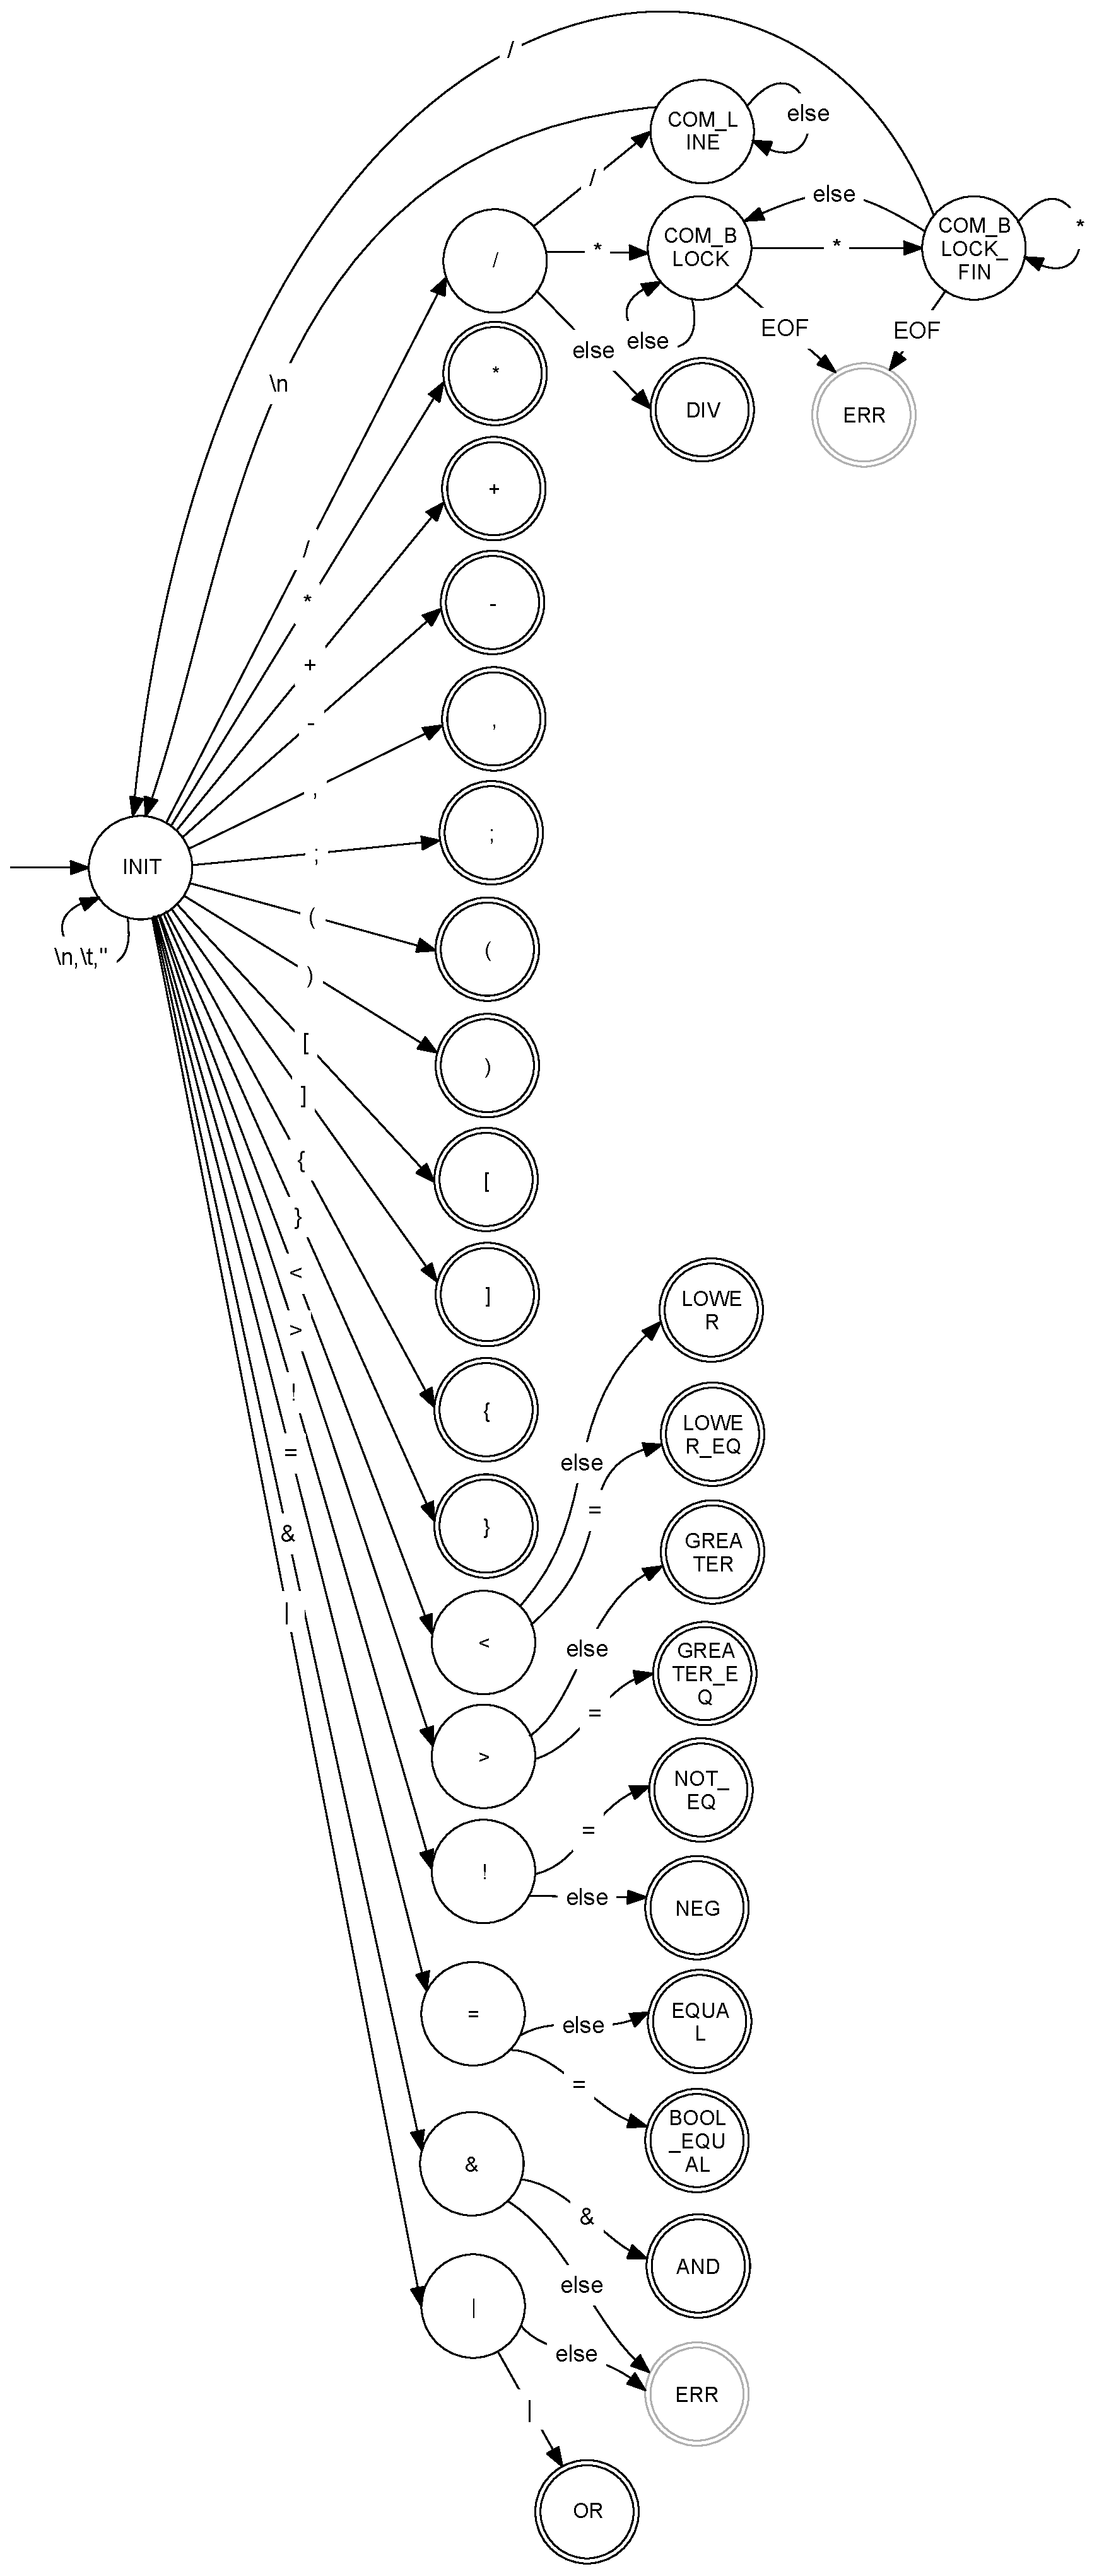
\includegraphics[scale=.31]{FSM_MAIN.eps}
	\caption{KA - hlavní schéma}
\end{figure}

\newpage
\begin{figure}[H]
	\centering
	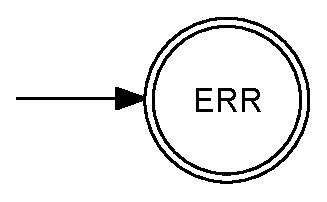
\includegraphics[scale=.31]{FSM_ERR.eps}
	\caption{KA - chyba}
\end{figure}

\begin{figure}[H]
	\centering
	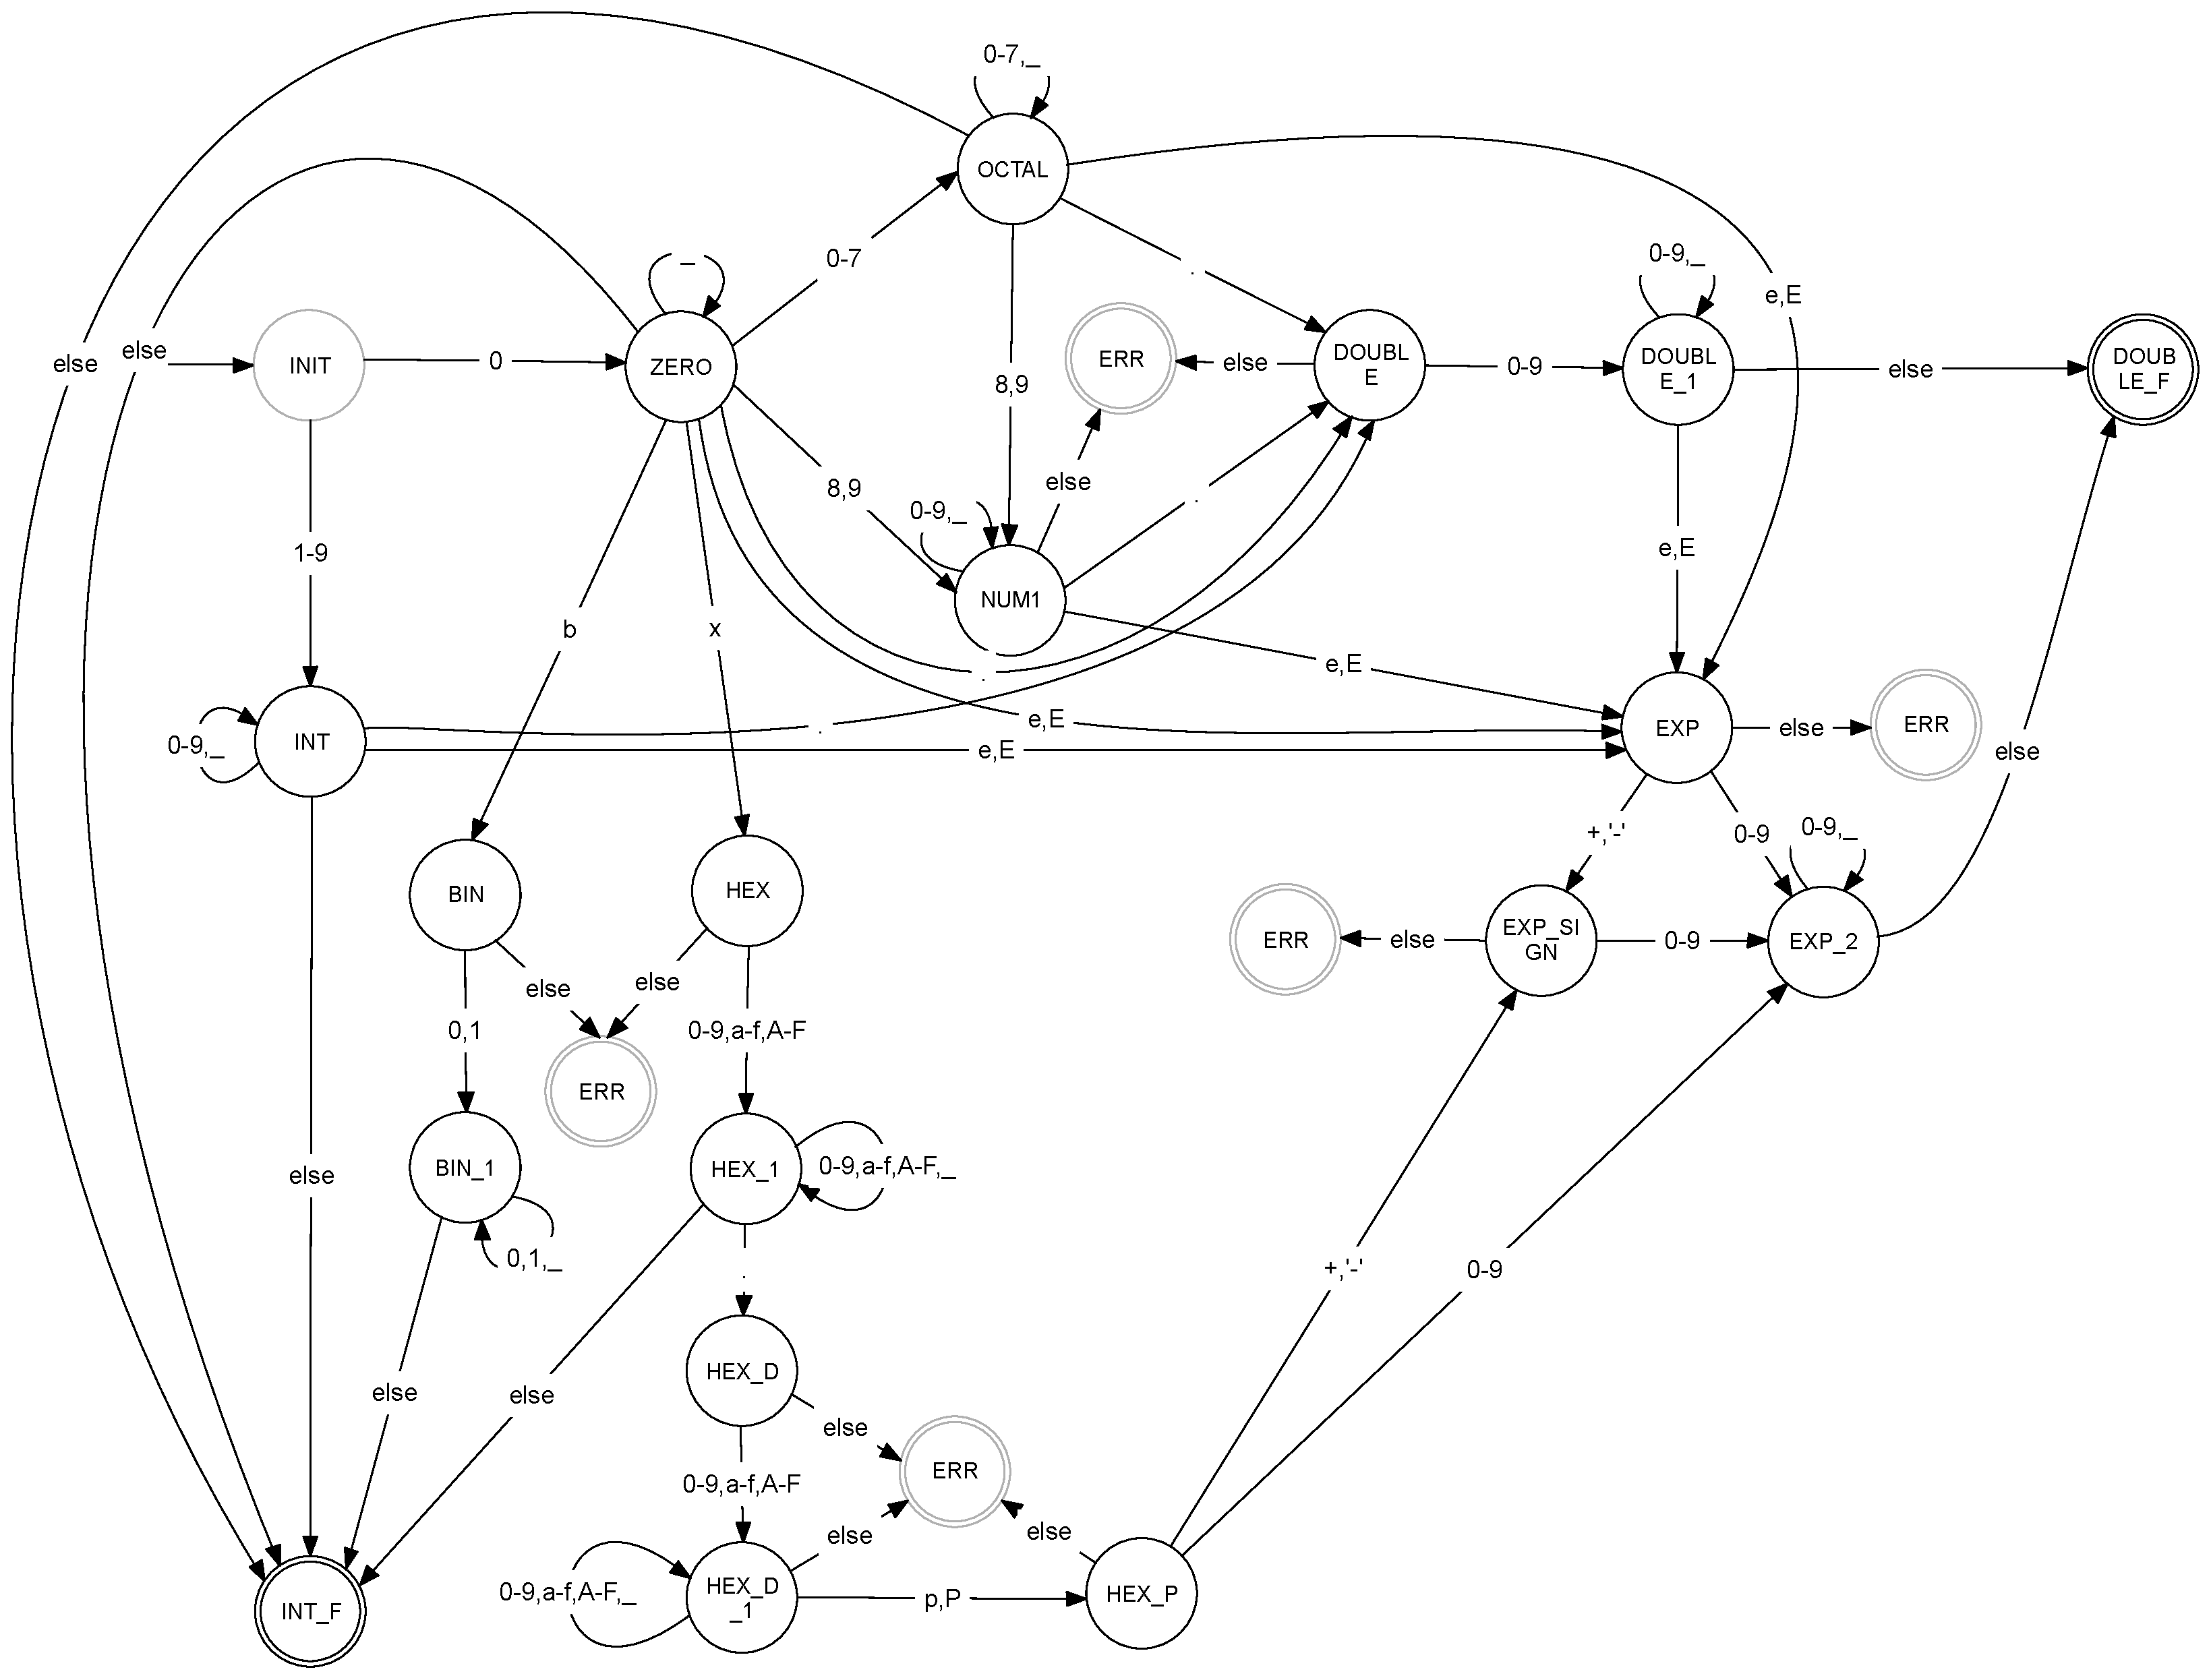
\includegraphics[scale=.31]{FSM_NUM.eps}
	\caption{KA - číslicový literál}
\end{figure}

\begin{figure}[H]
	\centering
	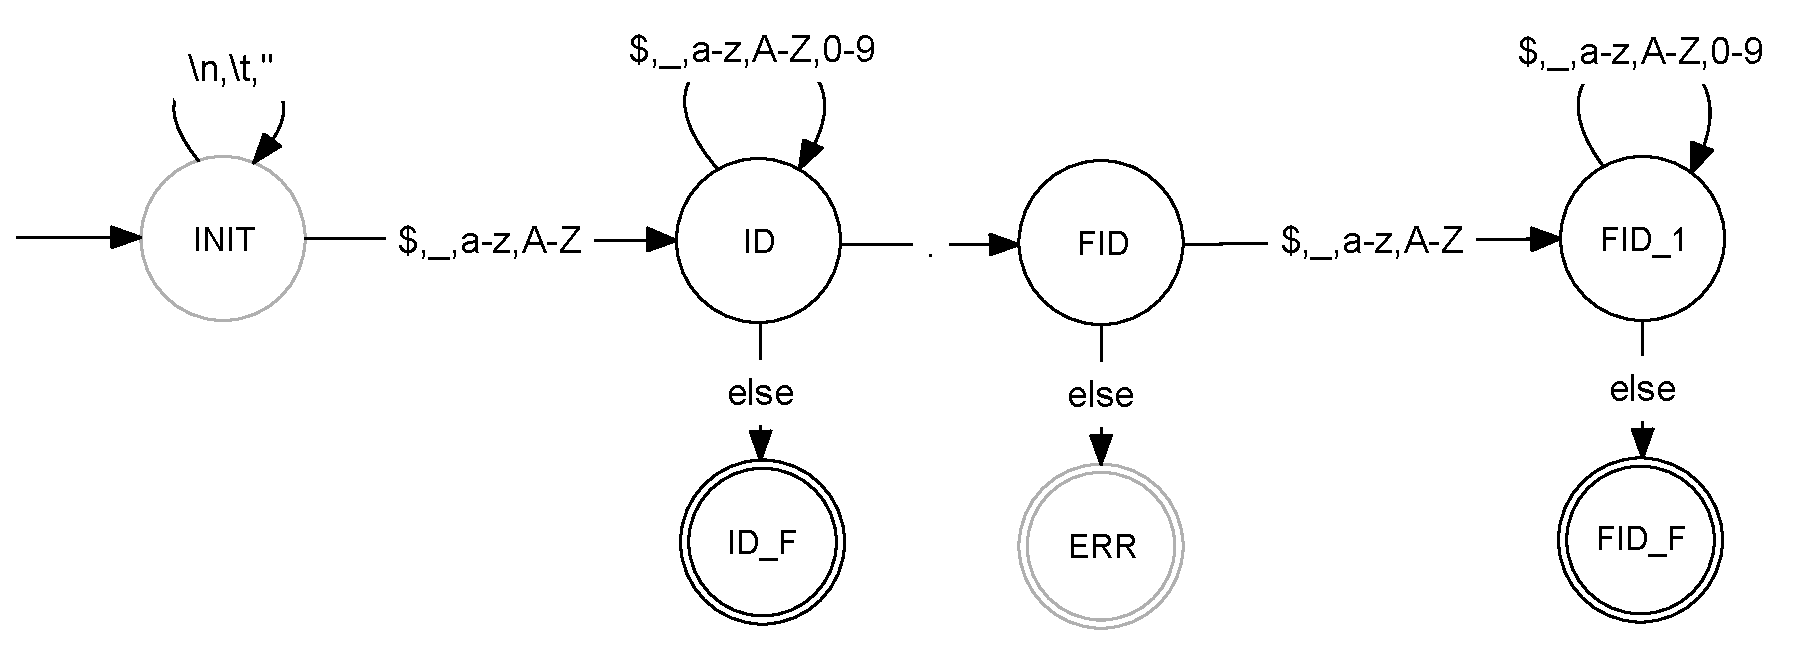
\includegraphics[scale=.31]{FSM_ID.eps}
	\caption{KA - identifikátor}
\end{figure}

\newpage
\begin{figure}[H]
	\centering
	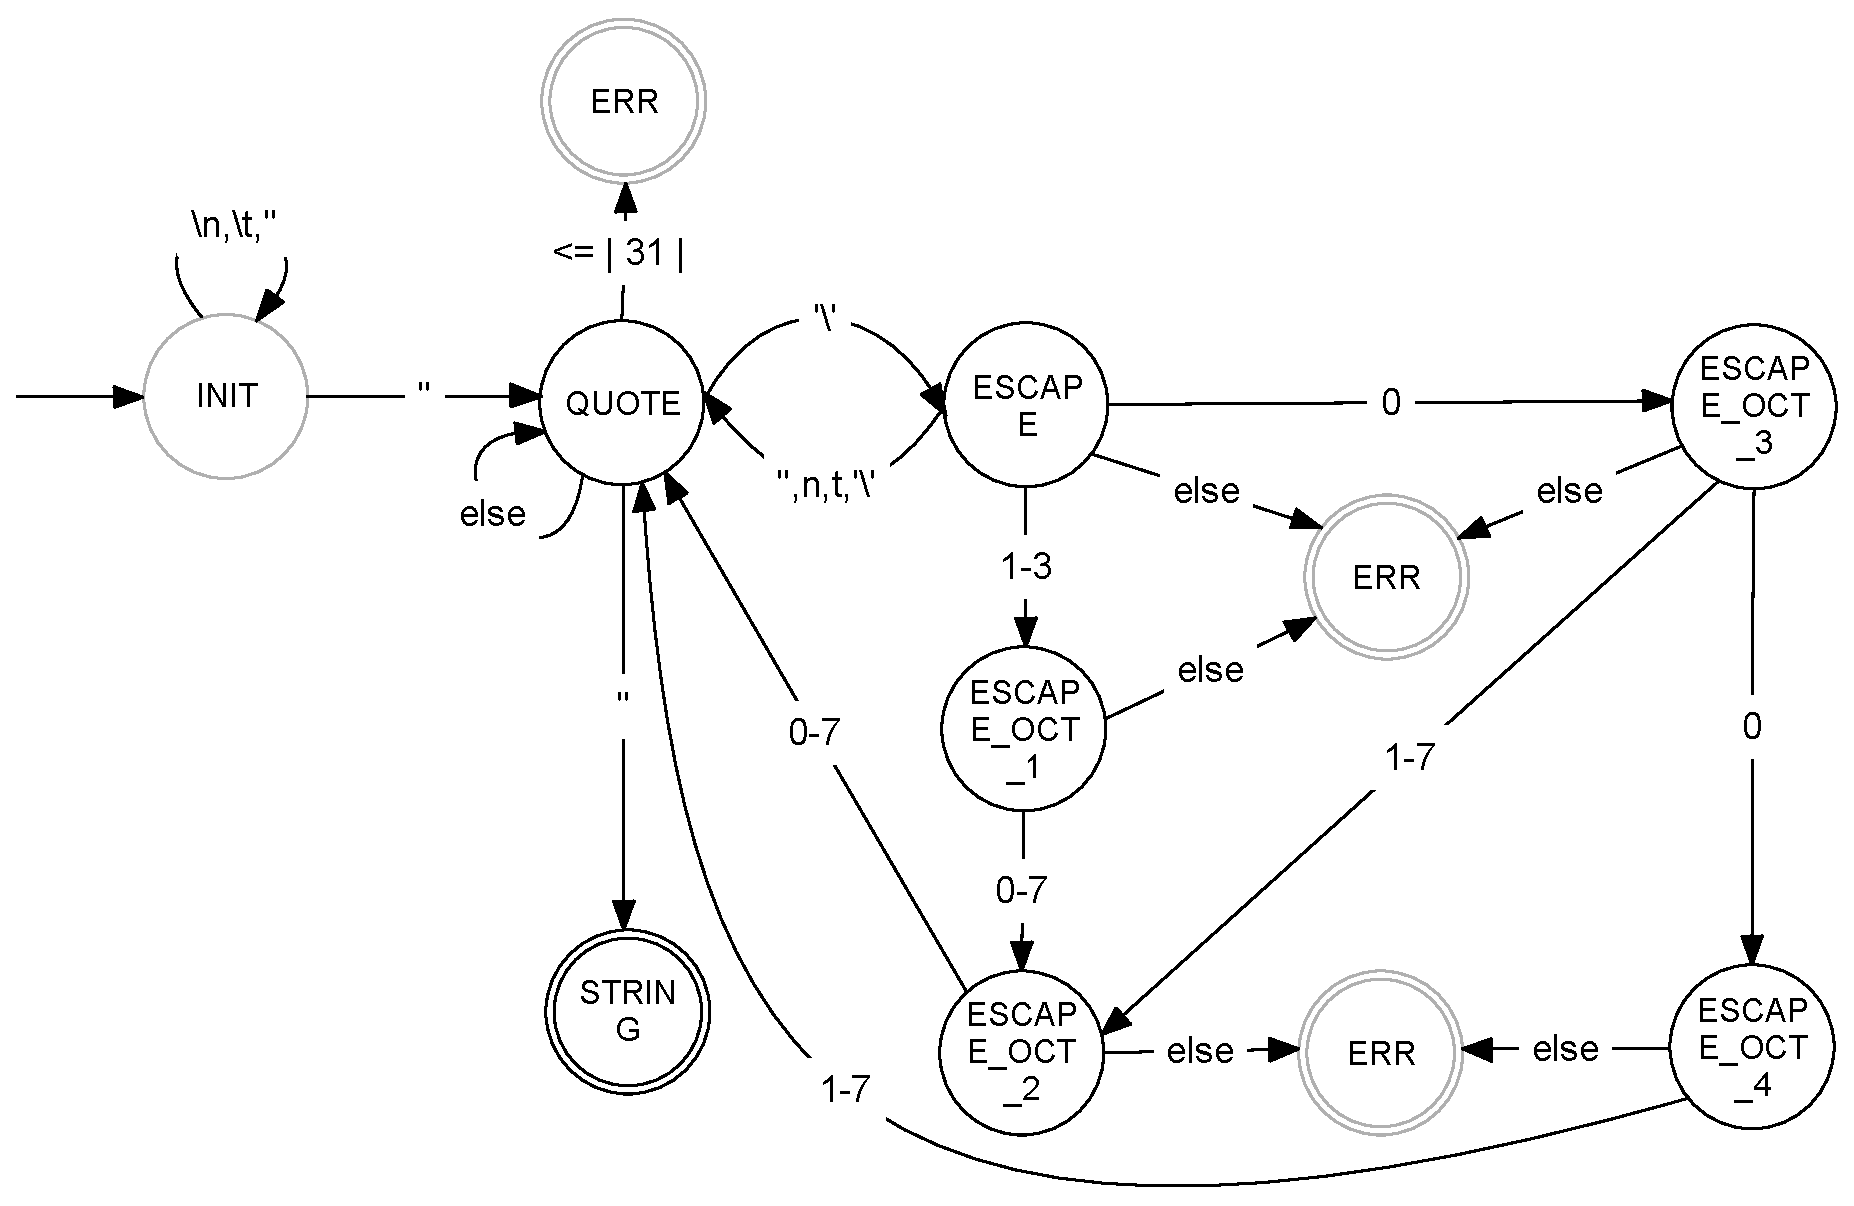
\includegraphics[scale=.31]{FSM_STRING.eps}
	\caption{KA - řetězec}
\end{figure}

\subsection{Precedenční tabulkaa}
\begin{figure}[H]
   \centering
   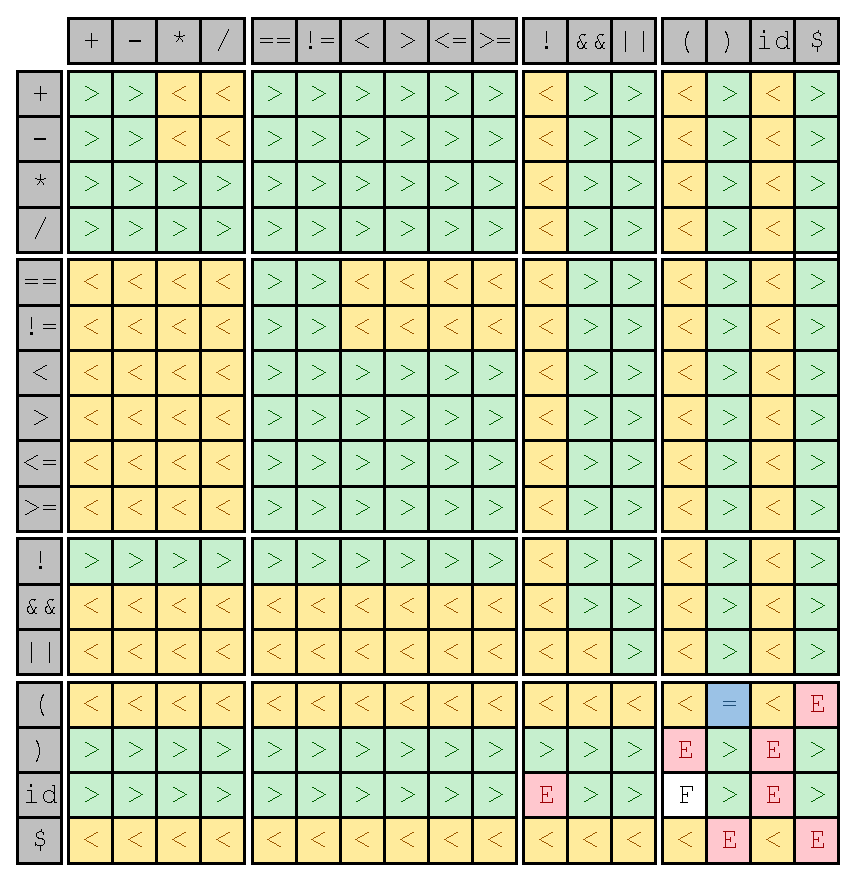
\includegraphics[]{precedence_tab.eps}
   \caption{Precedenční tabulka}
\end{figure}
\end{document}